\section{Zonky}
\label{analyza:zonky}

Přímé půjčky od lidí, kteří rádi pomohou. Jinak řečeno -- buďme lidští a vynechejme z~toho banky.

\subsection{Hlavní stránka}
Viz obrázek \ref{fig:zonky:home}.
\begin{figure}[h]
    \centering
    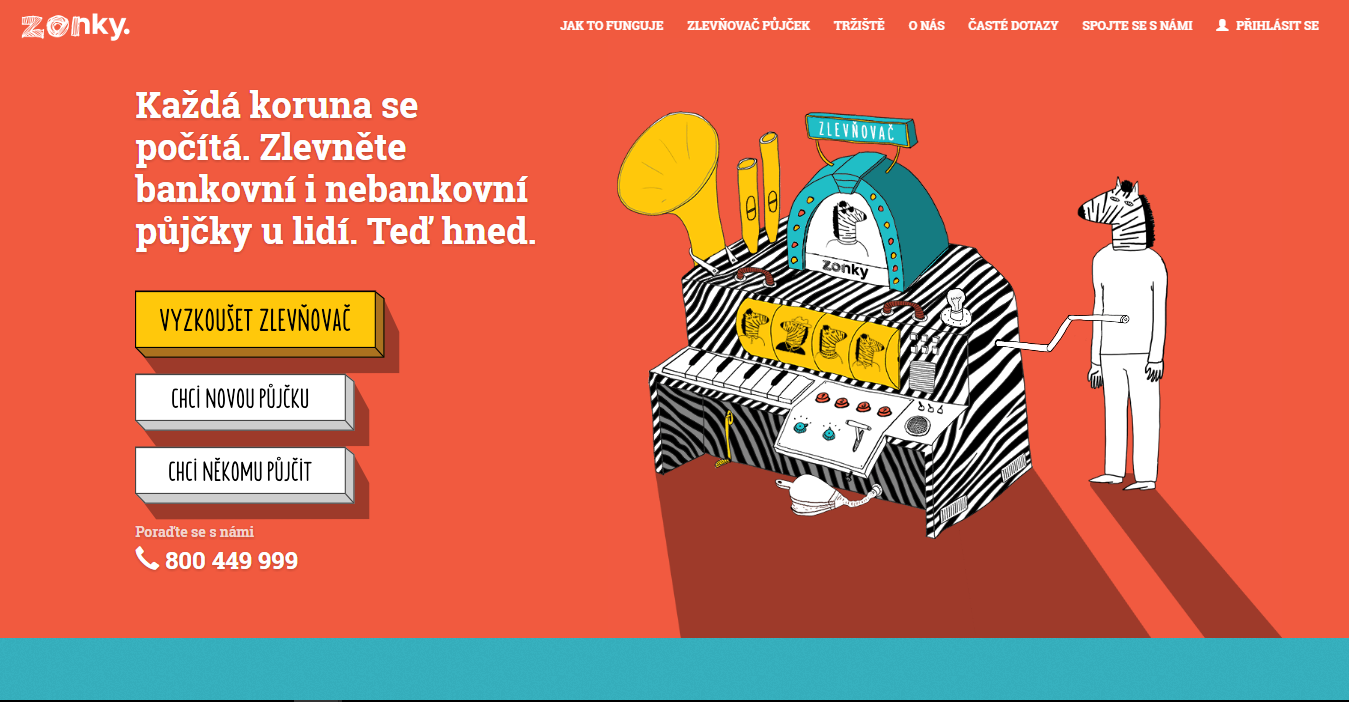
\includegraphics[width=1.0\textwidth]{media/zonky/home.png}
    \caption{Zonky.cz -- Hlavní stránka}
    \label{fig:zonky:home}
\end{figure}
\subsubsection*{Pozitiva}
\begin{itemize}
    \item[+] \textbf{Jednoduchost a přehlednost} -- Existence pouze pár tlačítek a jasná čitelnost všeho, co se na dané stránce nachází.
\end{itemize}
\subsubsection*{Negativa}
\begin{itemize}
    \item[-] \textbf{Zvuk} -- Velmi rušivý element, který se zvýší v~momentě, kdy má uživatel puštěnou na svém zařízení hudbu.
\end{itemize}


%%%%%%%%%%%%%%%%%%%%%%%%%%%%%%%%%%%%%%%%%%%%%%%%%%%%%%%%%%%%%%%%%%%%%%%%%%%%%%%%%%%%%%%%%%%%%%%%%%%%%%%%%%%%%%%%%%%%%%%%

\newpage
\subsection{Zlevnovač}
Viz obrázek \ref{fig:zonky:zlevnovac}. % a \ref{fig:zonky:zlevnovac2}.
\begin{figure}[h]
    \centering
    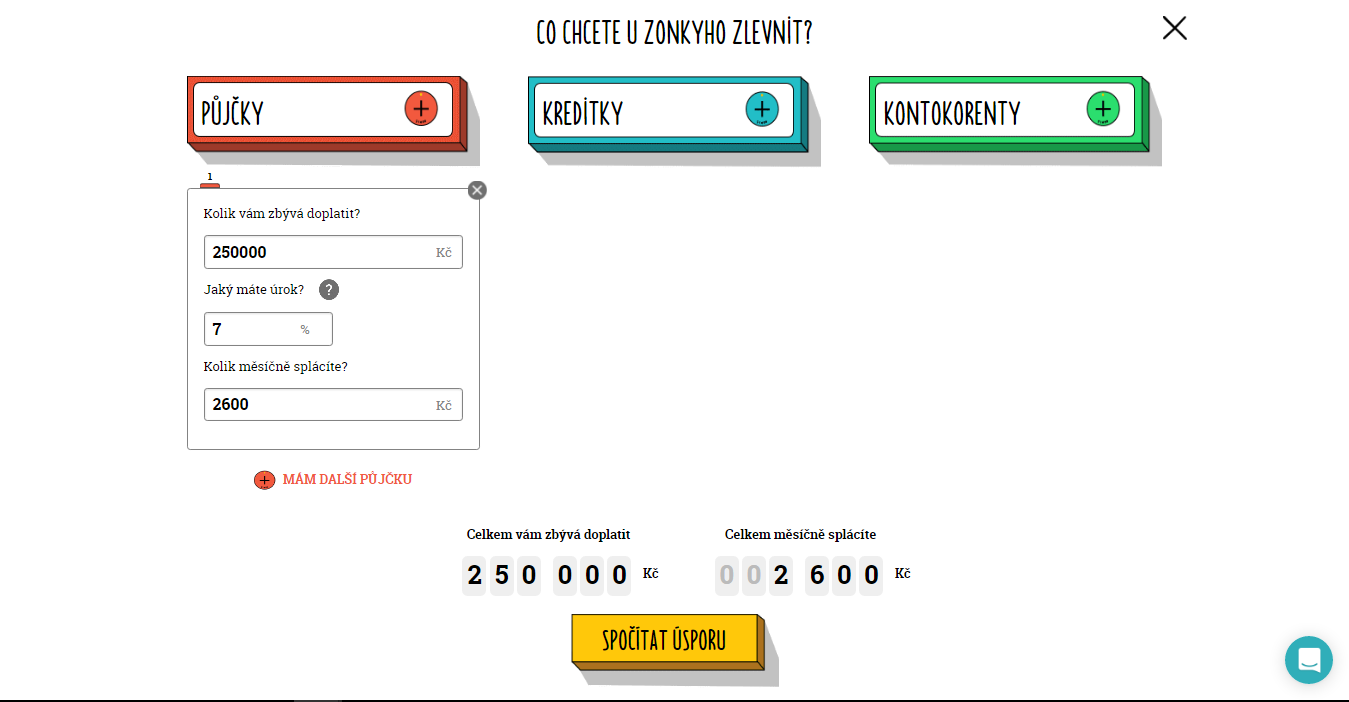
\includegraphics[width=1.0\textwidth]{media/zonky/zlevnovac.png}
    \caption{Zonky.cz -- Zlevňovač}
    \label{fig:zonky:zlevnovac}
\end{figure}
%\begin{figure}[h]
%    \centering
%    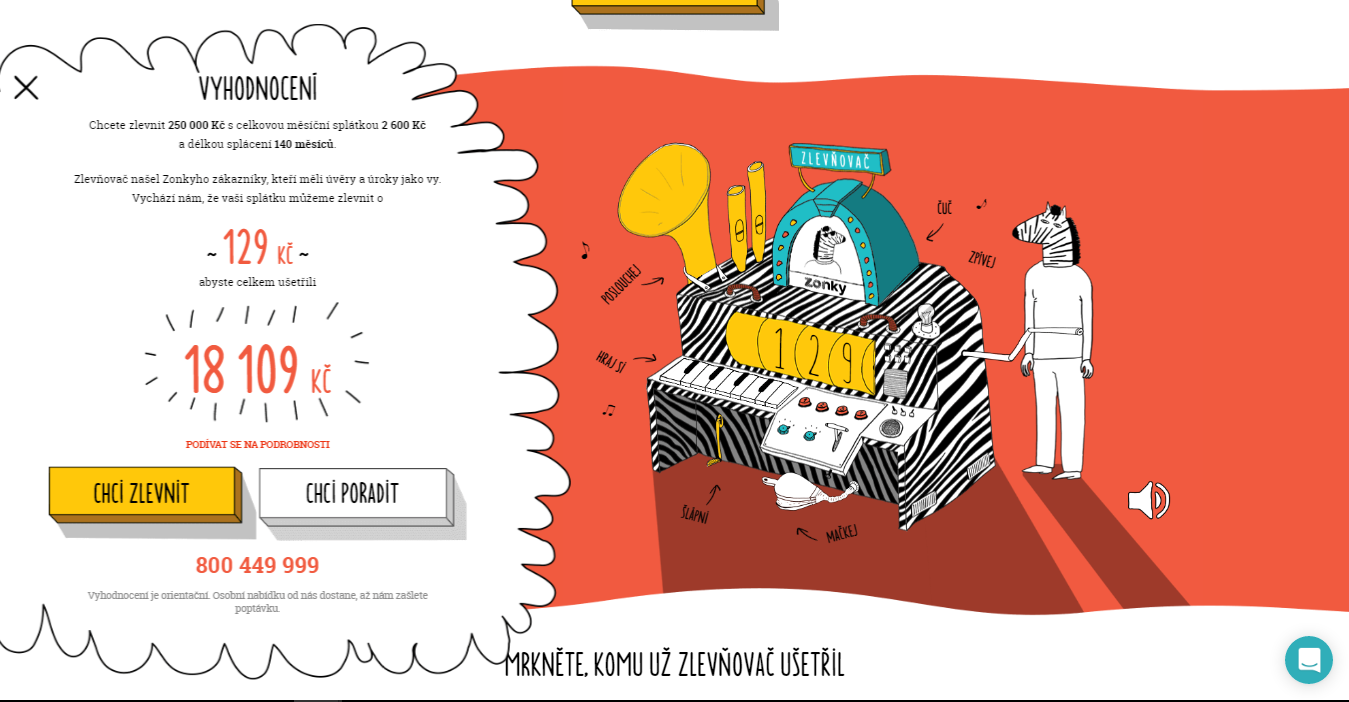
\includegraphics[width=1.0\textwidth]{media/zonky/zlevnovac2.png}
%    \caption{Zlevňovač na webu Zonky.cz 2}
%    \label{fig:zonky:zlevnovac2}
%\end{figure}
\subsubsection*{Pozitiva}
\begin{itemize}
    \item[+] \textbf{Jednoduchost a přehlednost} -- Opět jednoduché uživatelské rozhraní, ve kterém se nachází jen to potřebné.
    \item[+] \textbf{Vyhodnocení} -- Rychlý náhled na to, kolik uživatel ušetří, podaný pěknou a jasnou formou.
\end{itemize}
\subsubsection*{Negativa}
\begin{itemize}
    \item[-] \textbf{Zvuk}.
\end{itemize}


%%%%%%%%%%%%%%%%%%%%%%%%%%%%%%%%%%%%%%%%%%%%%%%%%%%%%%%%%%%%%%%%%%%%%%%%%%%%%%%%%%%%%%%%%%%%%%%%%%%%%%%%%%%%%%%%%%%%%%%%

\newpage
\subsection{Tržiště}
Viz obrázek \ref{fig:zonky:marketplace}.
\begin{figure}[h]
    \centering
    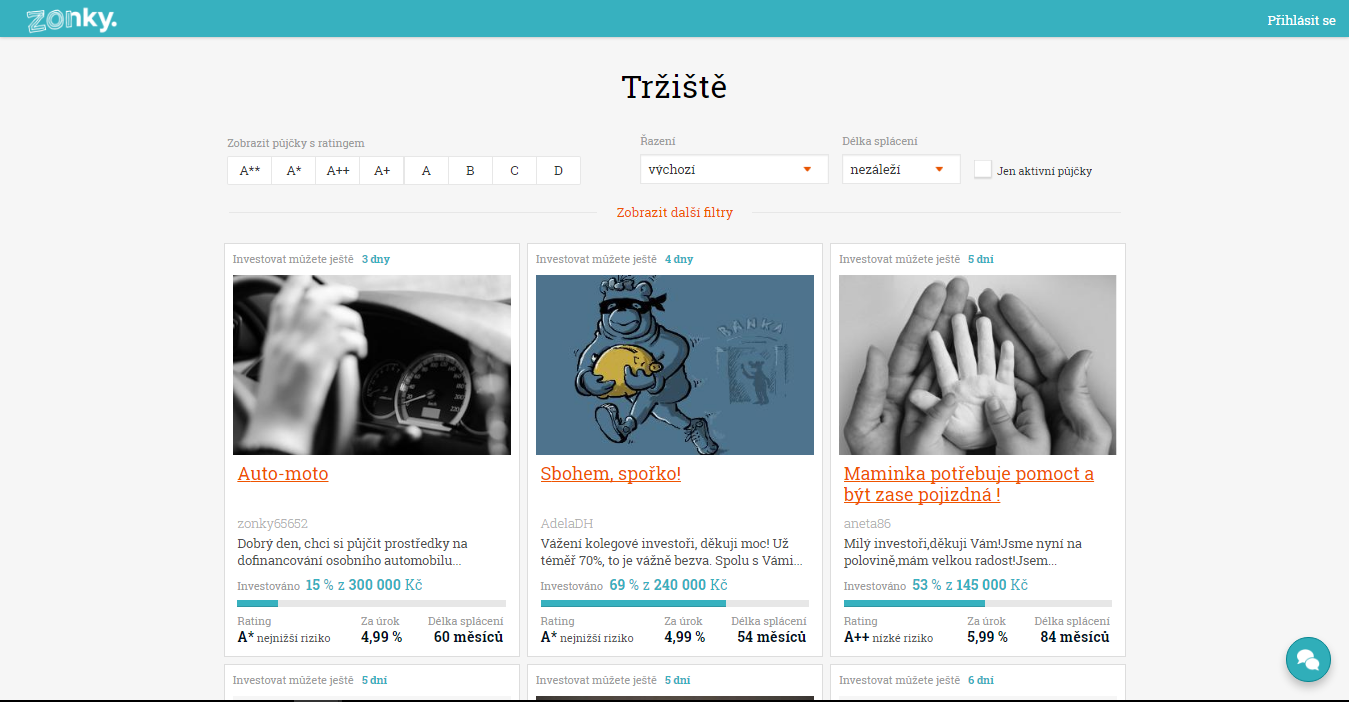
\includegraphics[width=1.0\textwidth]{media/zonky/marketplace.png}
    \caption{Zonky.cz -- Tržiště}
    \label{fig:zonky:marketplace}
\end{figure}
\subsubsection*{Pozitiva}
\begin{itemize}
    \item[+] \textbf{Informativnost} -- Krátký popis, rating\footnote{Rating určuje míru rizika.}, úrok a doba splácení je vše co uživatel na první pohled potřebuje.
    \item[+] \textbf{Filtry a řazení} -- Uživatel má šanci si rychle zobrazit nabídky, které ho zajímají.
\end{itemize}
\subsubsection*{Negativa}
\begin{itemize}
    \item[-] \textbf{Žádná negativa na této stránce nejsou pozorována.}
\end{itemize}


%%%%%%%%%%%%%%%%%%%%%%%%%%%%%%%%%%%%%%%%%%%%%%%%%%%%%%%%%%%%%%%%%%%%%%%%%%%%%%%%%%%%%%%%%%%%%%%%%%%%%%%%%%%%%%%%%%%%%%%%

\newpage
\subsection{Návodné a informativní stránky}
Viz obrázky \ref{fig:zonky:info}, \ref{fig:zonky:info2} a \ref{fig:zonky:info3}.
\begin{figure}[h]
    \centering
    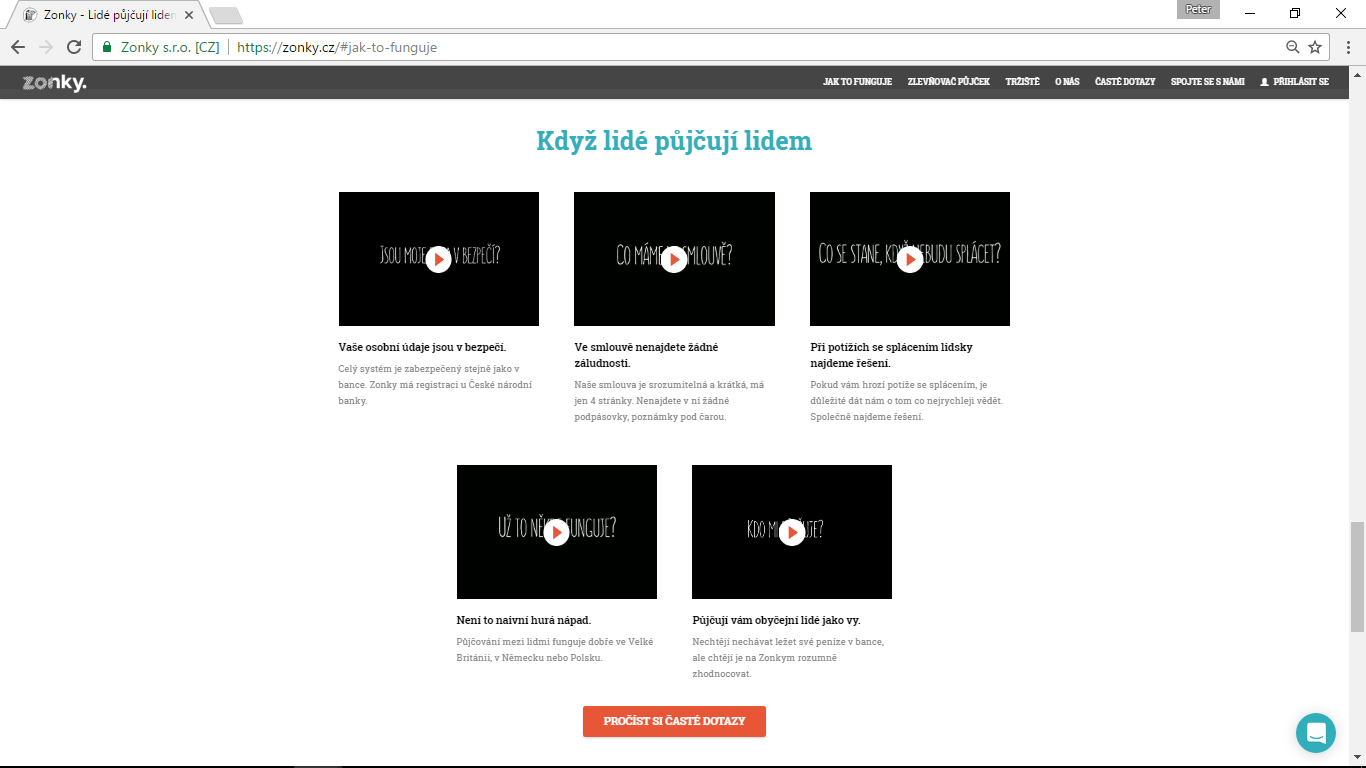
\includegraphics[width=1.0\textwidth]{media/zonky/info.png}
    \caption{Zonky.cz -- Když lidé půjčují lidem}
    \label{fig:zonky:info}
\end{figure}
\begin{figure}[h]
    \centering
    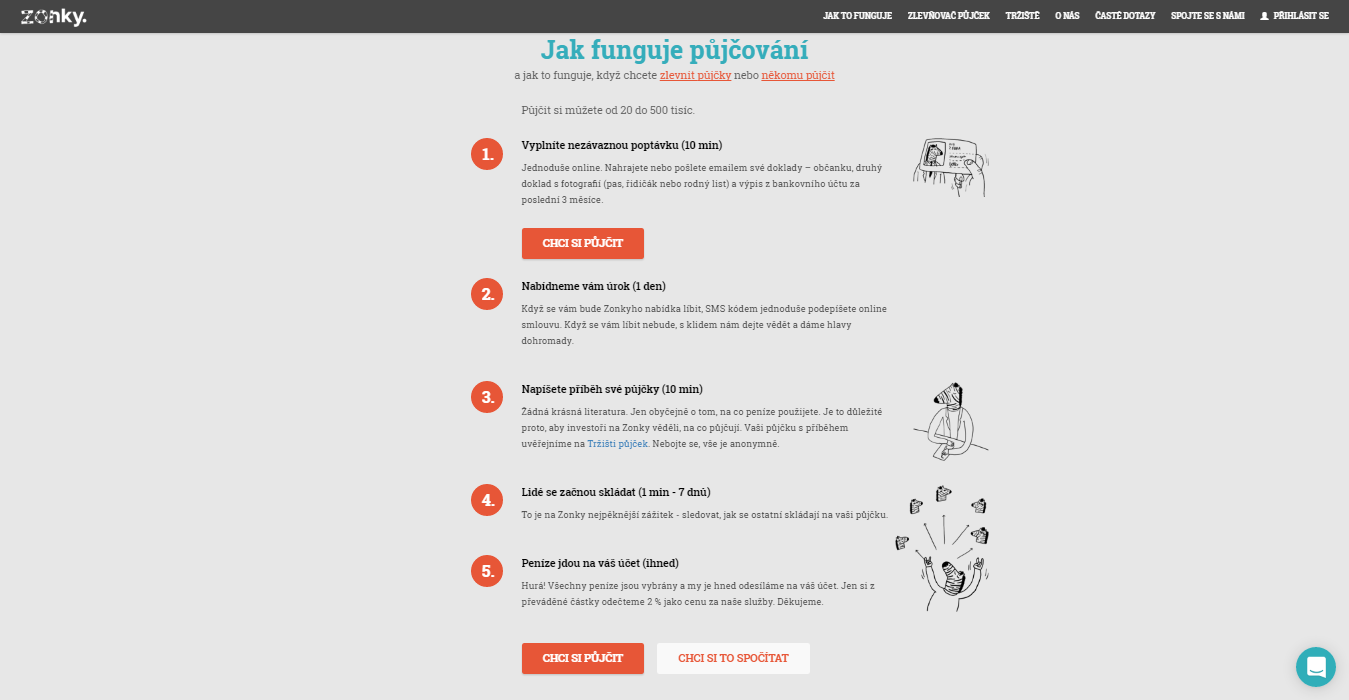
\includegraphics[width=1.0\textwidth]{media/zonky/info2.png}
    \caption{Zonky.cz -- Jak funguje půjčování}
    \label{fig:zonky:info2}
\end{figure}
\begin{figure}[h]
    \centering
    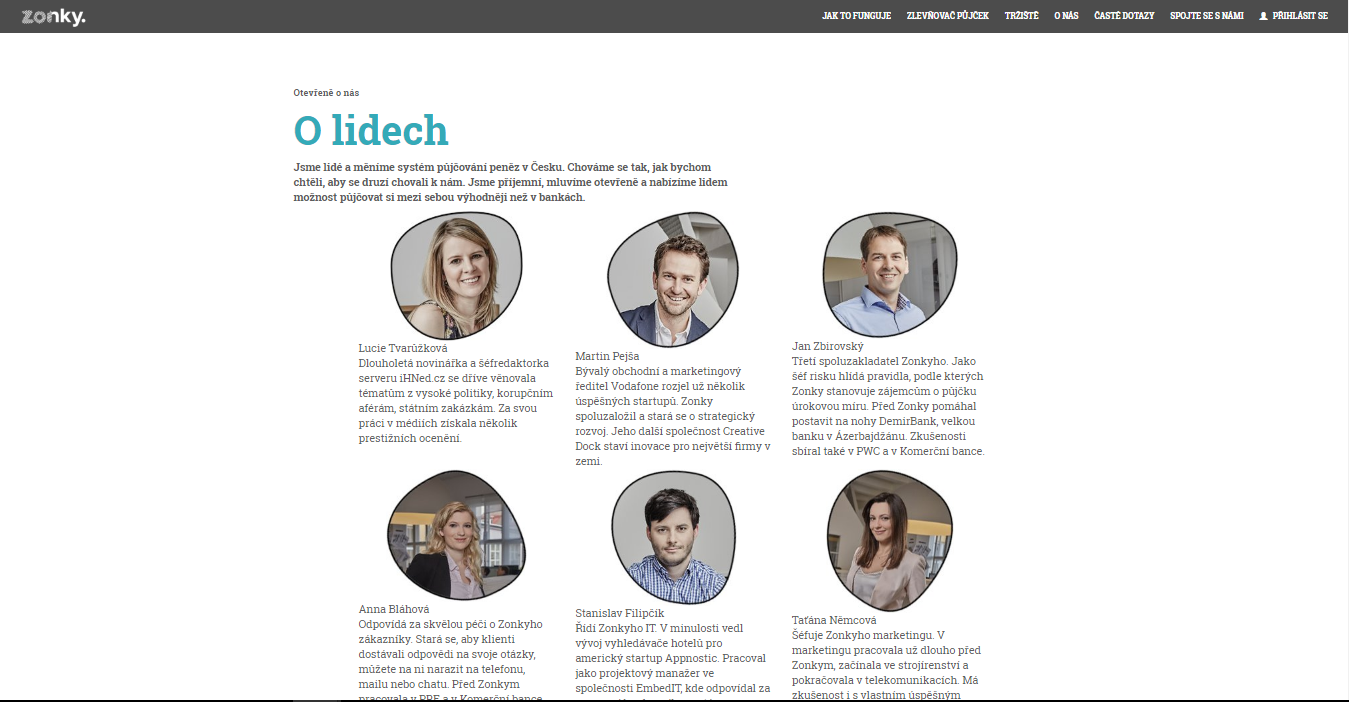
\includegraphics[width=1.0\textwidth]{media/zonky/info3.png}
    \caption{Zonky.cz -- O~lidech}
    \label{fig:zonky:info3}
\end{figure}
\subsubsection*{Pozitiva}
\begin{itemize}
    \item[+] \textbf{Uživatelská přívětivost} -- Informace jsou podány snadně, jednoduše a přehledně. Nic není zbytečně rozsáhlé.
\end{itemize}
\subsubsection*{Negativa}
\begin{itemize}
    \item[-] \textbf{Žádná negativa na těchto stránkách nejsou pozorována.}
\end{itemize}


%%%%%%%%%%%%%%%%%%%%%%%%%%%%%%%%%%%%%%%%%%%%%%%%%%%%%%%%%%%%%%%%%%%%%%%%%%%%%%%%%%%%%%%%%%%%%%%%%%%%%%%%%%%%%%%%%%%%%%%%

\subsection{Shrnutí}
Zonky.cz deklaruje, že chce pomoci lidem, resp. poskytuje možnost pro lidi pomáhat si navzájem. Stejná věc je očekávána i od aplikace vyvíjené v~této práci.

Pokud má aplikace pomáhat lidem, tak uživatelské rozhraní musí být příjemné na používání (to znamená \textbf{jednoduché a přehledné}). Stejně jako je to v~případě Zonky. V~každém zákoutí Zonky se k~uživateli dostává \textbf{dostatečné množství informací} (není zahlcen). \textbf{Přítomnost zvuku} je velmi odrazující.